\documentclass[12pt, a4paper]{article}
\title{Исследование разрешающей способности микроскопа методом Аббе (4.3.3)}
\author{Стеценко Георгий, Б02-312}
\date{}
% !TeX encoding = UTF-8

\usepackage{geometry}
\usepackage{amsmath, amsfonts, amssymb, amsthm} % стандартный набор AMS-пакетов для математ. текстов
\usepackage{mathtext}
\usepackage[utf8]{inputenc} % кодировка utf8
\usepackage[russian]{babel} % русский язык
\usepackage[pdftex,dvipsnames]{xcolor} % работа с цветами
\usepackage[pdftex]{graphicx} % графика (картинки)
\usepackage{tikz,pgfplots} % рисунки
\usepackage{indentfirst}
%\usepackage[labelfont=bf,labelsep=endash,skip=3pt]{caption} % подпись картинок
% \usepackage{fancyhdr,pageslts} % настройка колонтитулов
\usepackage{enumitem} % работа со списками
\usepackage{floatrow,multicol,multirow,longtable,hhline} % работа с таблицами
\usepackage{float,wrapfig} % плавающие объекты
\usepackage{tcolorbox} % рамка вокруг текста
%\usepackage[calc]{datetime2} % дата
\usepackage{bm} % жирное начертание в формулах
\usepackage{physics} % физический пакет
\DeclareMathAlphabet\mathbfcal{OMS}{cmsy}{b}{n}
\usepackage{pgfornament} % красивые рюшечки и вензеля
\usepackage{mdframed}
\usepackage{derivative}
\usepackage{mathrsfs} %EDS
\usepackage{soul} % strikethorugh
%\usepackage{boondox-cal}

% ----------------------------------------
% Настройка шрифта

% Просто закооментируйте следующую строчку, если не работает. Будет другой шрифт, правда :(
% \usepackage{pscyr}

% ----------------------------------------
% Стилевые настройки

\usepackage{boldline} % жирная линия после таблиц (чтобы не было ошибок, этот пакет должен подключаться именно тут!)
\floatsetup[table]{style=Plaintop,floatrowsep=qquad} % настройка оформления таблиц
\setlist[enumerate,itemize]{leftmargin=5mm,itemindent=10mm,itemsep=0mm,
listparindent=0em,labelsep=2mm,topsep=2mm,labelwidth=4mm} % настройки списков

\setlength{\columnsep}{0.5cm} % расстояние между колонками
\setlength{\parskip}{1pt} % расстояние до текста от колонтитула

%\usepackage{titlesec} % управление оформлением section
%\renewcommand{\thesection}{\Roman{section}}
%\titleformat{\section}[block]{\bfseries\large}{\thesection.}{5pt}{}

% ----------------------------------------
% Настройки полей
\geometry{
  left=10mm,
  top=10mm,
  right=10mm,
  bottom=15mm,
  marginparsep=0mm,
  marginparwidth=0mm,
  headheight=0pt,
  headsep=0pt,
footskip=20pt}

% ----------------------------------------
% Настройки колонтитулов и нумерации страниц
\pagenumbering{arabic}



\newcounter{ntask}
\setcounter{ntask}{0}


\newcommand{\arsh}{\mathrm{arsh} \,\,}
\newcommand{\arch}{\mathrm{arch} \,\,}
\newcommand{\arth}{\mathrm{arth} \,\,}
\newcommand{\arcth}{\mathrm{arcth} \,\,}
\renewcommand{\Re}{\operatorname{Re} \,}
\newcommand{\EDS}{\mathscr{E}}
\newcommand{\diffract}[1]{\frac{\mathrm{d}#1}{\mathrm{d}t}}

\newcommand{\kHz}{~\mathrm{kHz}}
\newcommand{\GHz}{~\mathrm{GHZ}}
\newcommand{\us}{~\mathrm{\mu s}}
\newcommand{\J}{\mathcal{J}}
\newcommand{\uA}{~\mathrm{\mu A}}
\newcommand{\mim}{~\mathrm{mm}}
\newcommand{\V}{\mathcal{V}}
\addto\captionsrussian{\def\refname{Источники}}

\begin{document}
\maketitle

\section{Аннотация}
В работе предлагается определить периоды сеток сначала по их спектру на
удалённом экране, затем по увеличенному с помощью модели микроскопа изображению
сеток на экране и, наконец, по результатам измерения разрешающей способности
микроскопа, наблюдать явления саморепродукции, пространственной фильтрации и
мультиплицирования.

\section{Теоретические сведения}

Для иммерсионного микроскопа разрешающая способность объектива при
некогерентном освещении $$ \ell_{\min } \approx \frac{0.61 \lambda}{n \sin u}
$$ где $u$ -- апертурный угол объектива микроскопа (угол между оптической осью
и лучом, направленным из центра объекта в край линзы).

Метод Аббе для оценки разрешающей способности состоит в разделении хода лучей
на две части: сначала рассматривается картина в задней фокальной плоскости $F$
объектива; она называется первичным изображением или фурье-образом. Это
первичное изображение рассматривается как источник волн (согласно принципу
Гюйгенса-Френеля), создающий изображение в плоскости $P_{2}$, сопряжённой
плоскости предмета - вторичное изображение. Первичное изображение есть картина
дифракции Фраунгофера (на дифракционной решётке), если её период $d$, то для
направления максимальной интенсивности $\varphi_{m}$ $$ d \sin \varphi_{m}=m
    \lambda $$ При этом проходят пучки только с $\varphi_{m}<u .$ Можно условием
разрешения считать, что $u>\varphi_{1}$, иначе говоря $$ \sin u \geq \lambda /
    d $$ Или $$ d \geq \frac{\lambda}{\sin u} \approx \frac{\lambda}{D / 2 f} $$
где $D-$ диаметр линзы, $f-$ фокусное расстояние. Двумерную решётку можно
рассматривать как две перпендикулярные друг другу, для максимумов которых
выполняется соотношение $$ d \sin \varphi_{x}=m_{x} \lambda, \quad d \sin
    \varphi_{y}=m_{y} \lambda $$

\newpage
\section{Экспериментальная установка}
\begin{figure}[H]
    \centering
    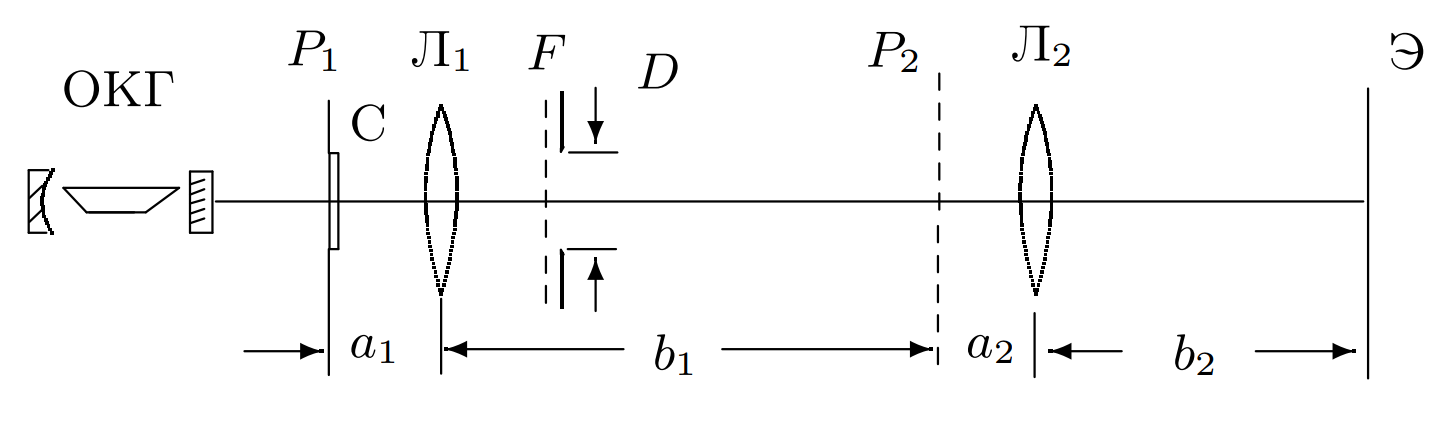
\includegraphics[width = 0.7\textwidth]{pics/setup.png}
    \caption{Схема экспериментальной установки — модель проекционного
        микроскопа}
    \label{fig:setup}
\end{figure}

Схема установки приведена на Рис. \ref{fig:setup}. Предметом $P_{1}$ служат
сетки в кассете $C$. Линза Л1 -- длиннофокусная, а Л2 -- короткофокусная. В F
Устанавливаются диафрагмы D, с помощью сеток с разными периодами $d$ и щелевой
диафрагмы можно проверить третье соотношение. Период сеток может быть измерен
либо по расстоянию между дифракционными максимумами на экране, либо по
увеличенному с помощью микроскопа изображению сетки на экране. Пространственную
фильтрацию (получение наклонного изображение решётки) можно получить с помощью
подбора угла наклона и ширины вспомогательной щели.

\section{Методика измерений и результаты}
\subsection{Определение периода решёток по их пространственному спектру}

Закрепим кассету с двумерными решётками (сетками) вблизи выходного окна лазера.
Вращая наружное кольцо кассеты, пронаблюдаем на удалённом экране дифракционные
картины для разных сеток. Для определения расстояния между соседними
дифракционными максимумами измерим расстояние между удалёнными друг от друга
горизонтальными максимумами и число промежутков между ними. На погрешность
измерения размеров также то, что максимумы не являются в точности точками.
\begin{table}[H]
    \centering
    \caption{Определение периодов решёток в кассете}
    \begin{tabular}{|c|c|c|c|}
        \hline
                                         & 1               & 2               & 3              \\
        \hline
        \multicolumn{4}{|c|}{ВЕРХ}                                                            \\
        \hline
        расстояние, $\mathrm{mm}$        & $215 \pm 3   $  & $259 \pm 3$     & $ 172 \pm 3$   \\
        число клеток                     & 3               & 9               & 12             \\
        период решётки, $\mathrm{\mu m}$ & $10.00\pm 0.14$ & $24.8 \pm 0.3$  & $49.9 \pm 0.9$ \\
        \hline
        \multicolumn{4}{|c|}{НИЗ}                                                             \\
        \hline
        расстояние, $\mathrm{mm}$        & $215  \pm 3$    & $174 \pm 3$     & $200 \pm 3$    \\
        число клеток                     & 3               & 6               & 14             \\
        период решётки, $\mathrm{\mu m}$ & $10.00\pm 0.14$ & $24.7 \pm 0.4 $ & $50.1 \pm 0.8$ \\
        \hline
    \end{tabular}
\end{table}

Зная, что длина волны лазера $\lambda = 530~\mathrm{nm}$, а расстояние от
экрана до решётки измерено с помощью засечек на оптическом столе: $L = (1350\pm
    2)~\mathrm{mm}$, можно найти период решётки.

\subsection{Определение периода решёток по изображению, увеличенному с помощью
    модели микроскопа}

Соберём модель микроскопа, добавив линзы согласно Рис. 1. Фокусные расстояния
линз $F_{1}= 110$ mm, $F_{2}= 25$ mm. Измеряем необходимые расстояния: $$
    \begin{aligned}
        a_{1}       & = 120  \pm 10~\mathrm{mm}, \\
        a_{2}+b_{1} & = 455 \pm 10~\mathrm{mm},  \\
        b_{2}       & = 815 \pm 10~\mathrm{mm},
    \end{aligned}
$$

Погрешности здесь обусловлены неточностями в положениях сеток и линз. Из
формулы тонкой линзы $a_{2}=\frac{b_{2} F_{2}}{b_{2}-F_{2}}=(25.79\pm 0.01)$
mm, следовательно $b_{1}= 430\pm 10$ mm. Увеличение микроскопа $
    \Gamma=\frac{b_{1} b_{2}}{a_{1} a_{2}}=113 \pm 10$.

Здесь $d$ определялось по формуле $d=\frac{\Delta x}{\Gamma}$. Обратим
внимание, что значения периодов решётки совпадают в пределах погрешности.
\begin{table}[H]
    \centering
    \begin{tabular}{|c|c|c|c|c|}
        \hline
        реш. & $\Delta m$ & $l$, мм & $d,~\mathrm{\mu m}$ & $\varepsilon_d$, \% \\ \hline
        1    & 30         & 36      & $10.6  \pm 0.6$     & 5                   \\ \hline
        2    & 12         & 35      & $25.8 \pm 1.5$      & 6                   \\ \hline
        3    & 15         & 87      & $51.3 \pm 1.5$      & 3                   \\ \hline
    \end{tabular}
    \caption{Периоды дифракционных решеток}
    \label{table:ampd}
\end{table}
Видно, что в пределах погрешности периоды решёток совпали.

\subsection{Определение разрешающей способности микроскопа}

С помощью откалиброванных сеток определяется разрешающая способность
микроскопа. Для этого в задней фокальной плоскости $F$ объектива
устанавливается щелевая диафрагма с микрометрическим винтом и подбирается её
минимальный размер, при котором ещё видно изображение сетки на экране (щель
пропускает максимумы с $m = 0, \pm 1$). По размеру диафрагмы и фокусному
расстоянию объектива рассчитывается апертурный угол $u$ и проверяется
соотношение Аббе.

Измерения приведены в таблице \ref{tab:micro}.

\begin{table}[H]
    \centering
    \begin{tabular}{|p{2cm}|p{2cm}|p{2cm}|p{2cm}|p{2cm}|}
        \hline Решётка & $D$, мм & $d,~\mathrm{\mu m}$ \\ \hline
        1              & >4      & 10                  \\ \hline
        2              & 2,21    & 25                  \\ \hline
        3              & 1,03    & 50                  \\ \hline
    \end{tabular}
    \caption{Минимальное расстояние, разрешаемое микроскопом}
    \label{tab:micro}
\end{table}

По полученным данным, был построен график на рис. \ref{gr}.

\begin{figure}[H]
    \centering
    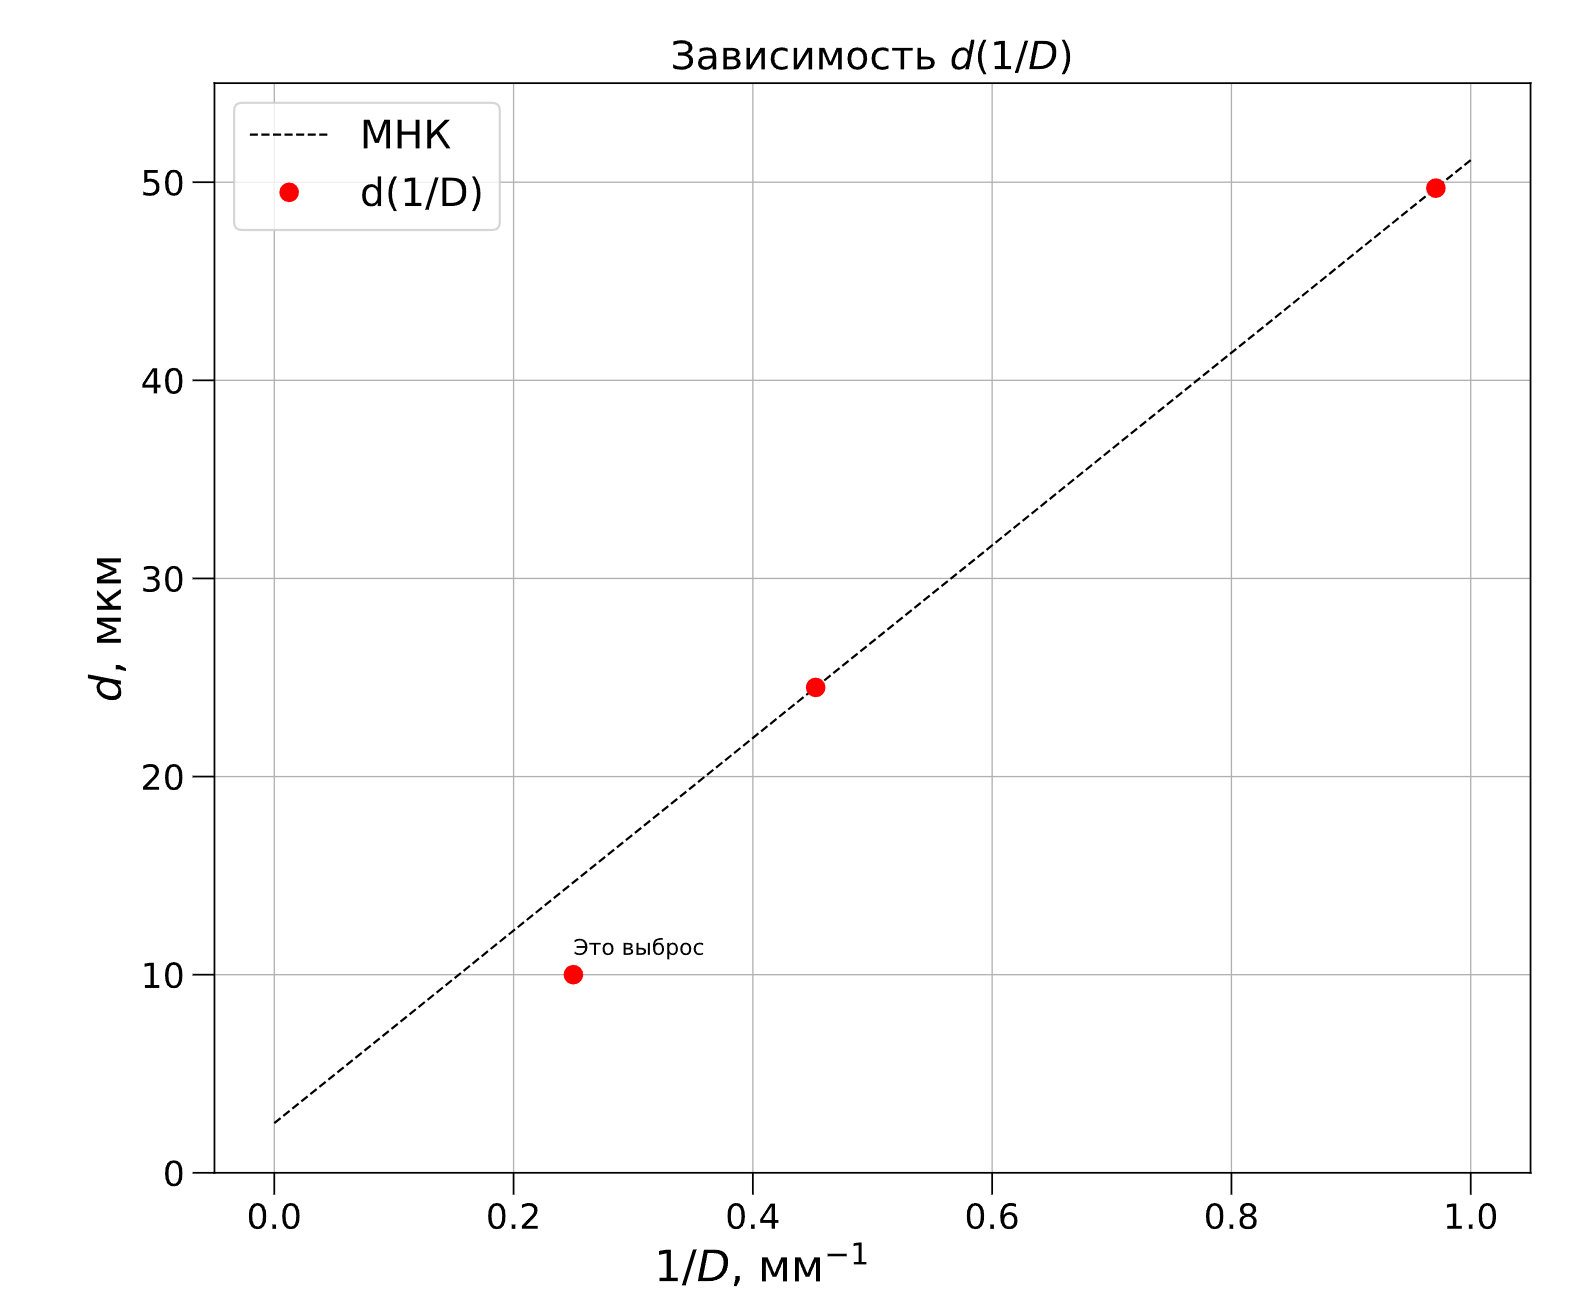
\includegraphics[scale=0.65]{pics/plot.png}
    \caption{График зависимости $d(1/D)$}
    \label{gr}
\end{figure}

<<Выброс>> на графике обусловлен органичением шкалы микрометра, что оставляет
валидными лишь 2 точки. По полученным данным сложно что-либо сказать о
справедливости теории Аббе.

\subsection{Пространственная фильтрация и мультиплицирование}

В процессе проведения опытов по пространственной фильтрации и
мультиплицированию были получены следющие фотографии.
\begin{figure}[H]
    \begin{minipage}{0.2\textwidth}

    \end{minipage}
    \begin{minipage}{0.3\textwidth}
        \centering
        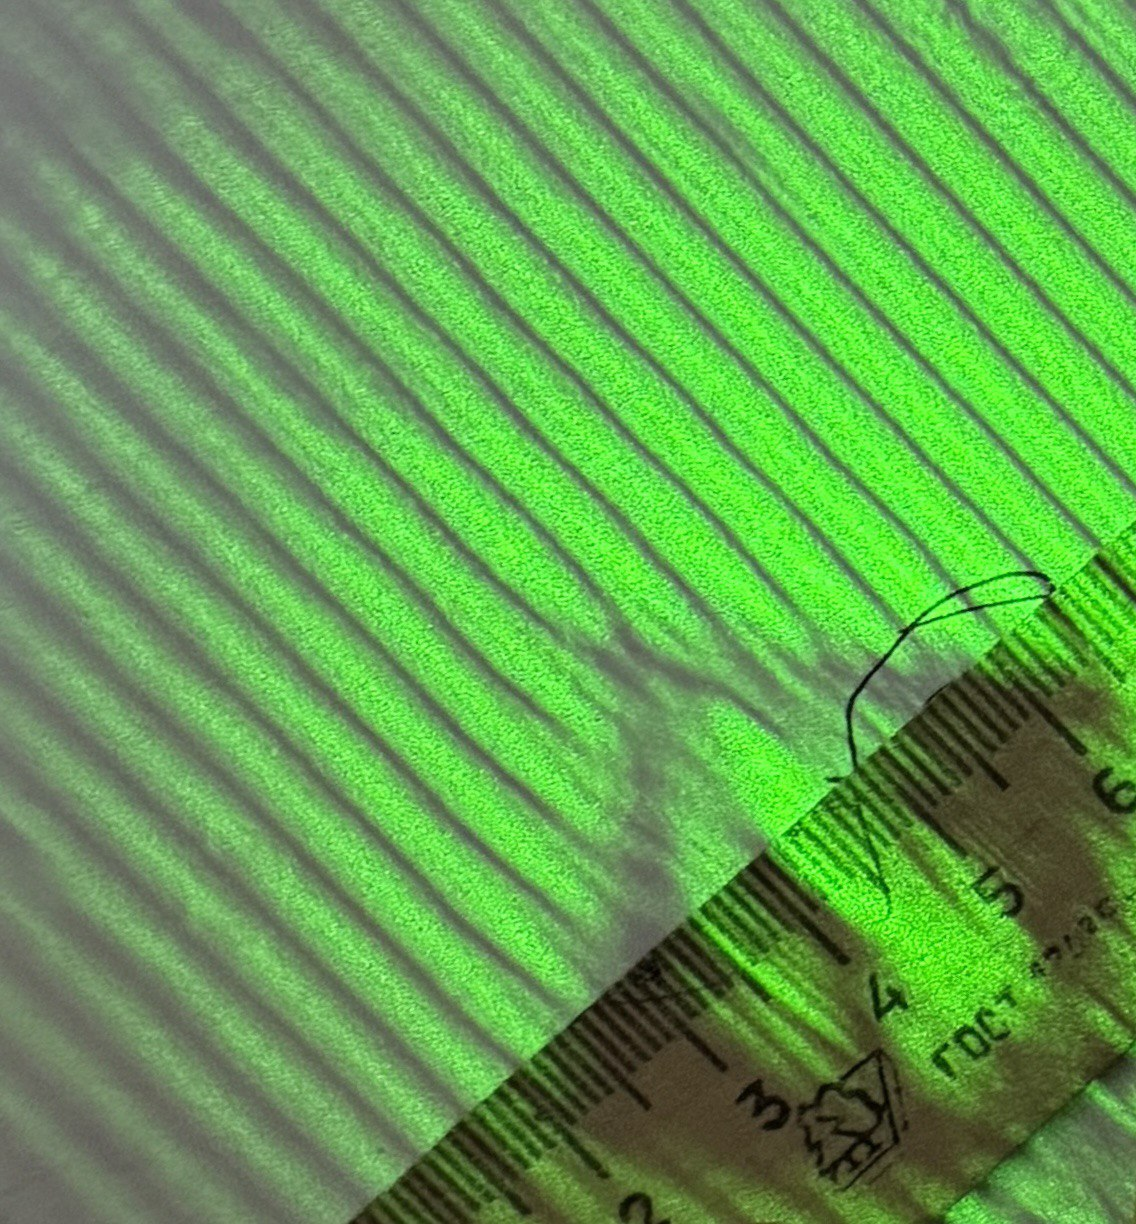
\includegraphics[height=\textwidth]{pics/diag.jpg}

    \end{minipage}
    \begin{minipage}{0.3\textwidth}
        \centering
        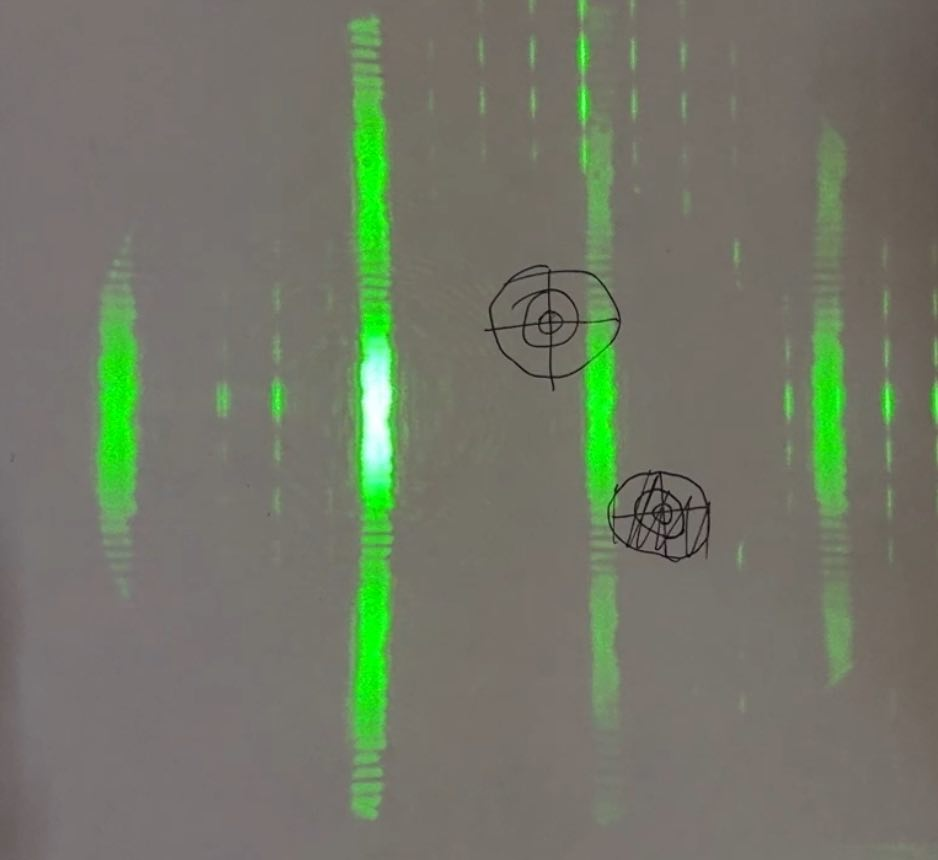
\includegraphics[height=\textwidth]{pics/mult.jpg}

    \end{minipage}
    \begin{minipage}{0.2\textwidth}

    \end{minipage}
    \hfill
    \caption{Слева -- результат пространственной фильтрации для $m_x = m_y$,
        справа -- результат мультиплицирования изображения щели}
\end{figure}
\section{Вывод}

По измерениям спектров получилось определить дифракционные углы и по
теоретическим формулам рассчитать периоды решеток. Полученные данные сошлись с
результатами, полученными по измерениям увеличенных с помощью микроскопа
изображений сеток.

\end{document}
